 \subsection{HPS beamline}
 
The Hall-B beam line, magnetic elements, beam profile monitors, and beam position and current monitors, upstream of the HPS setup will be used as is (after slight modifications for 12 GeV). The only modification needed for the upstream part of the beam line is the addition of a collimator upstream of the Hall-B tagger magnet. The role of the collimator is to prevent direct beam exposure of the Si-tracker in an event of beam excursions when high intensity beam can move up or down from the nominal position. The collimators, which  can be a $1$ cm thick tungsten plates with different size oval holes (as the beam profile) can be incorporated into the Hall-B photon tagger radiator ladder that provides vertical alignment. Horizontal alignment of the whole system will be needed for fine tuning of the collimator position relative to the beam. After the HPS setup, there will be two beamlines, the electron beam line that will transport electron beam to the Hall-B electron beam dump, and a photon beam line that will transport photon beam generated in the target to a photon beam dump mounted on the space frame. Electron beam will be transported in the vacuum alway through to the beam dump. The photon beam after the vacuum chamber through the last chicane dipole will go to the dump in Helium bag. There will be H-corrector installed on the electron line after the HPS chicane to compensate any possible mis-steering of the beam in the chicane, to make sure that the electron beam stays on the original beamline to the dump. Before the dump a YAG viewer will be used to monitor beam position. Before and after energizing the chicane, beam position on the dump monitor must stay unchanged.  
 
 \subsubsection{Layout of the HPS setup} 
 
The HPS experiment will use the same three magnet chicane that was used for the CLAS Two Photon Exchange experiment (TPE). The layout of the beam line and the chicane is shown in Figure \ref{fig:ebeam}. The Hall B pair spectrometer magnet, 18D36 (pole length $91.44$ cm, gap $45.72\times 15.24$ cm$^2$, max-field $1.5$ T), will serve as the analyzing magnet. The dipole field direction (Y) is perpendicular to the horizontal (XZ) plane. The Hall B �Frascati� H magnets (pole length $50$ cm, gap $21\times 8.25$ cm$^2$, max-field $1.2$ T) will be used as the first and the last dipoles of the chicane. The analyzing magnet will be operated at a $0.25$ T-m field for $1.1$ GeV, a $0.5$ T-m field for $2.2$ GeV, and a $1.5$ T-m field for $6.6$ GeV running. The two bending magnets will be set to  $0.125$ T-m, $0.25$ T-m, and $0.75$ T-m fields, respectively. The distance between centers of the magnets will be about $50$ cm bigger than it was for the TPE run. The location of the analyzing magnet along the beam will be exactly at the same place as for the TPE run. In transverse direction it will be displaced to beam left by $\sim 11$ cm in order to optimize the detector acceptance for e$^+$ and e$^-$, see Figure \ref{fig:ebeamt}.
 
 \begin{figure*}[!ht]
%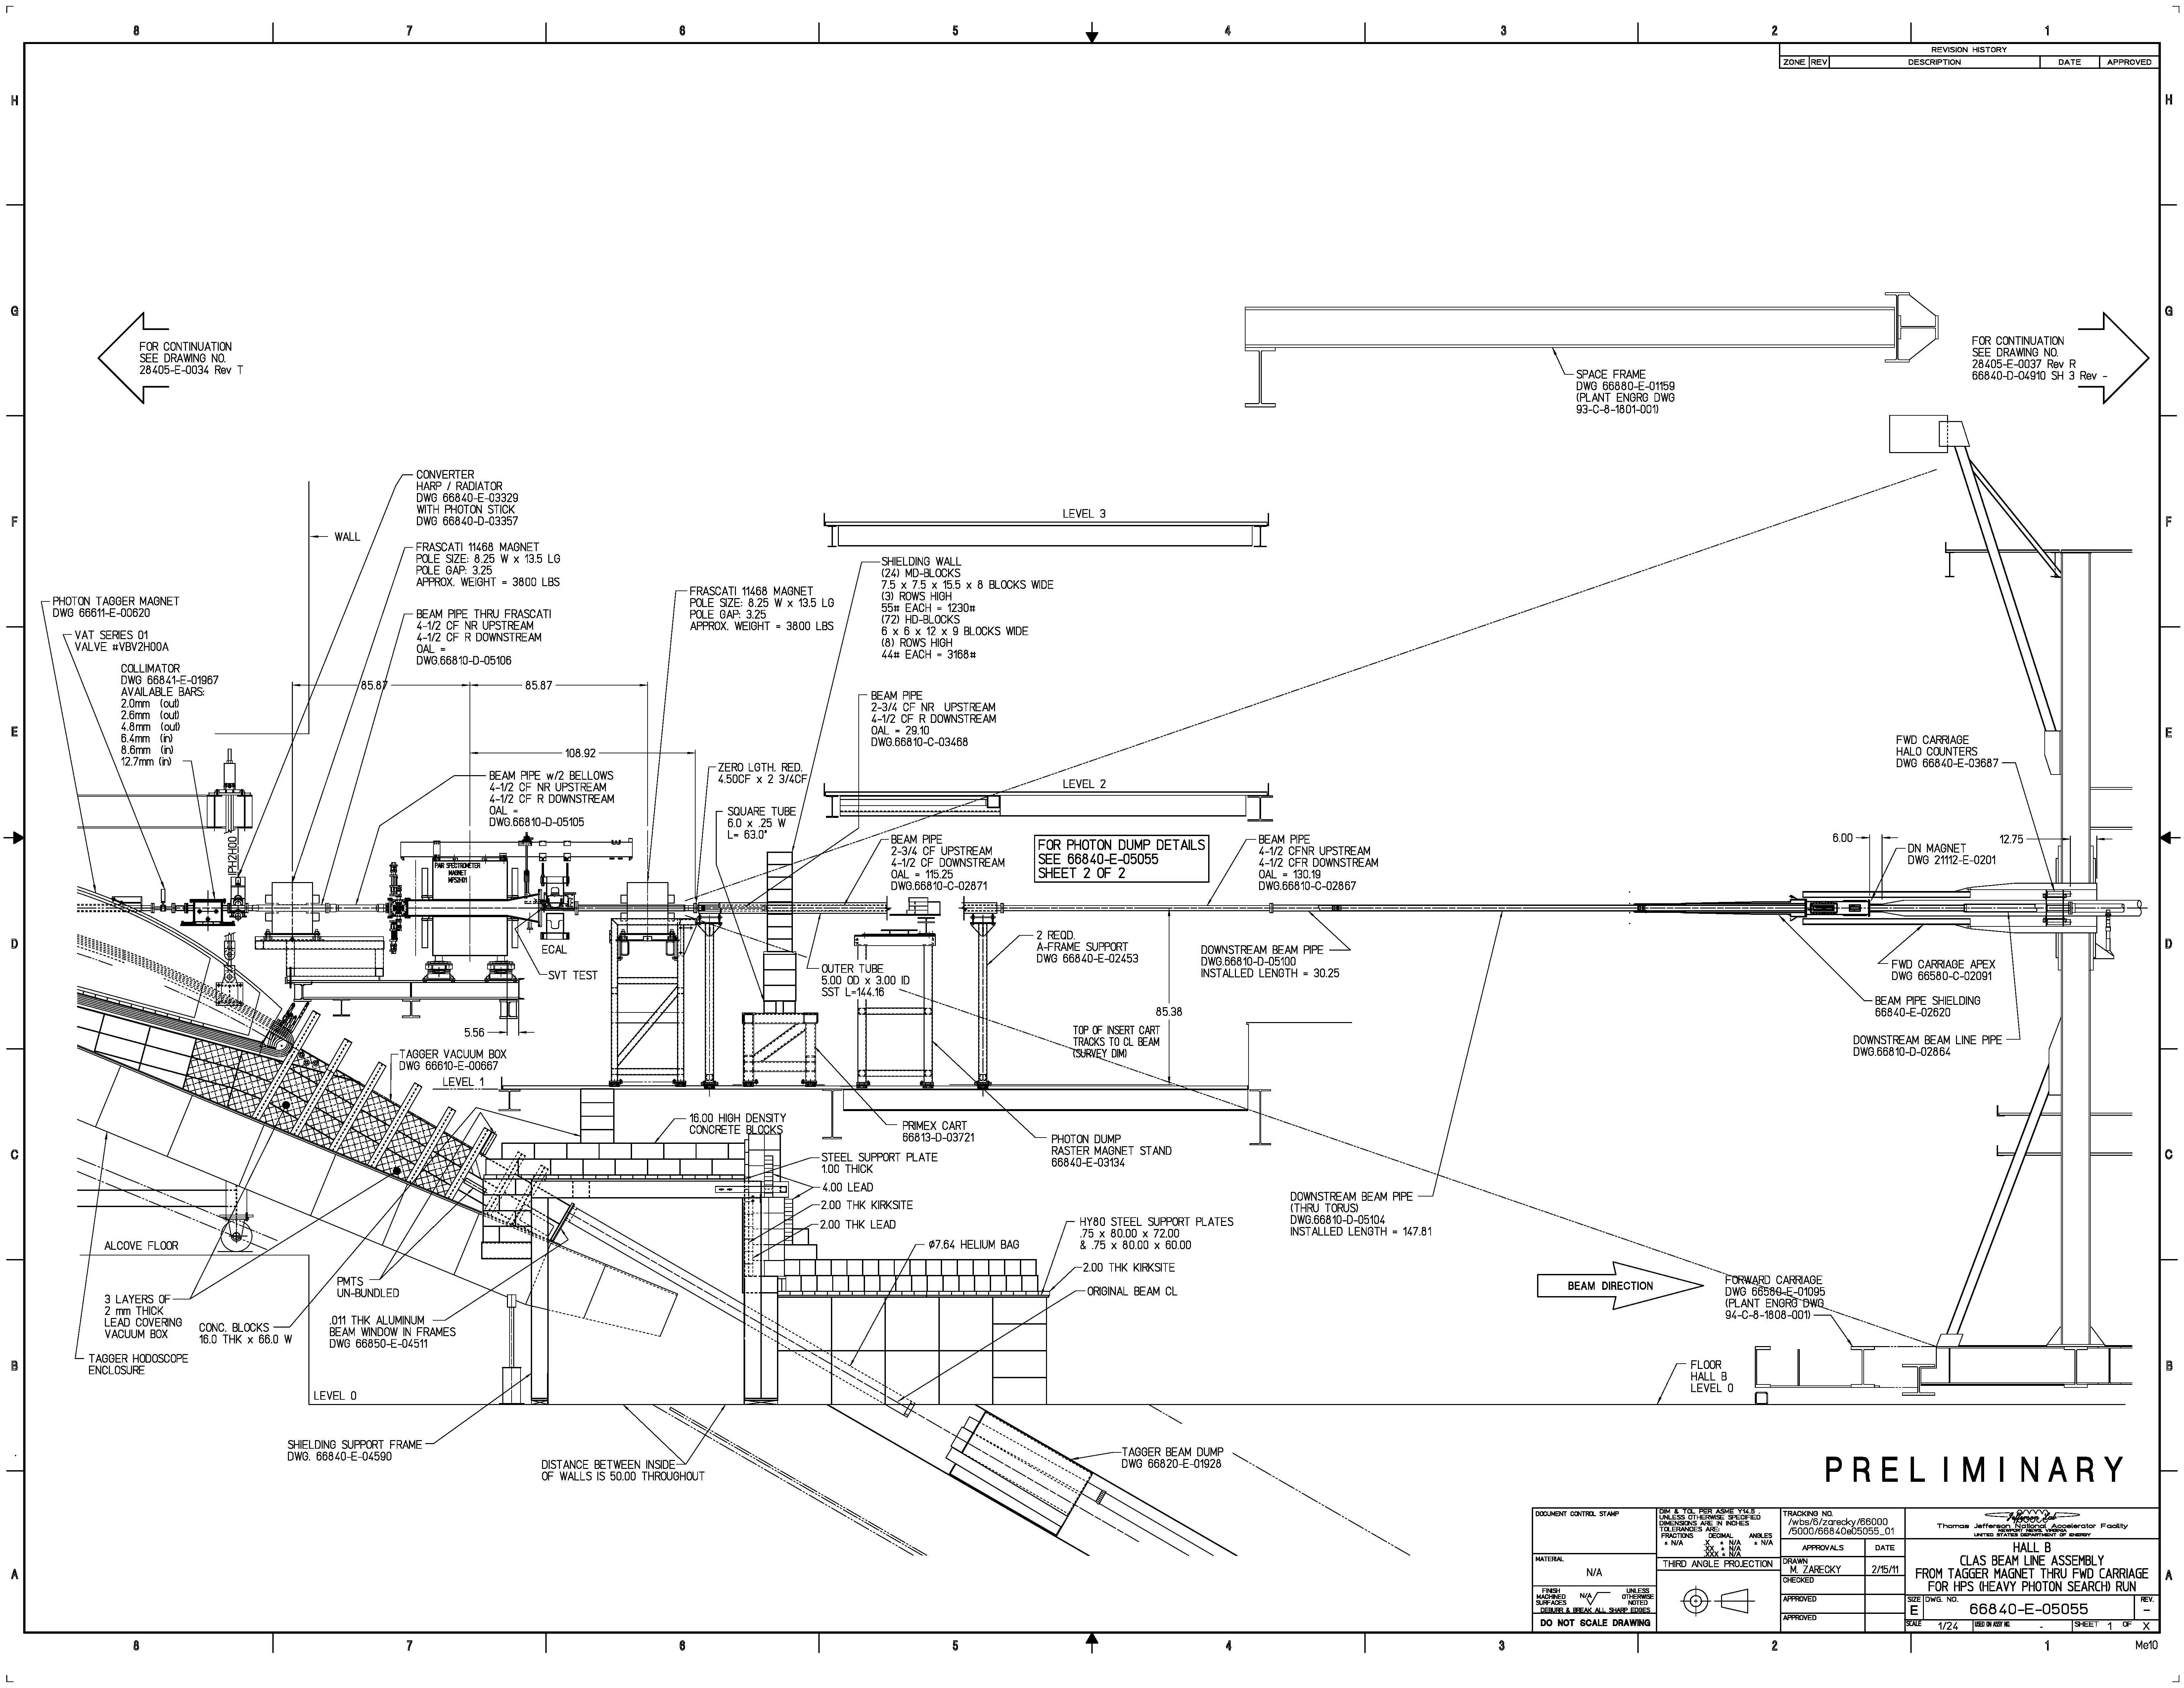
\includegraphics[scale=0.18]{beamline/05055-01_NT.pdf}
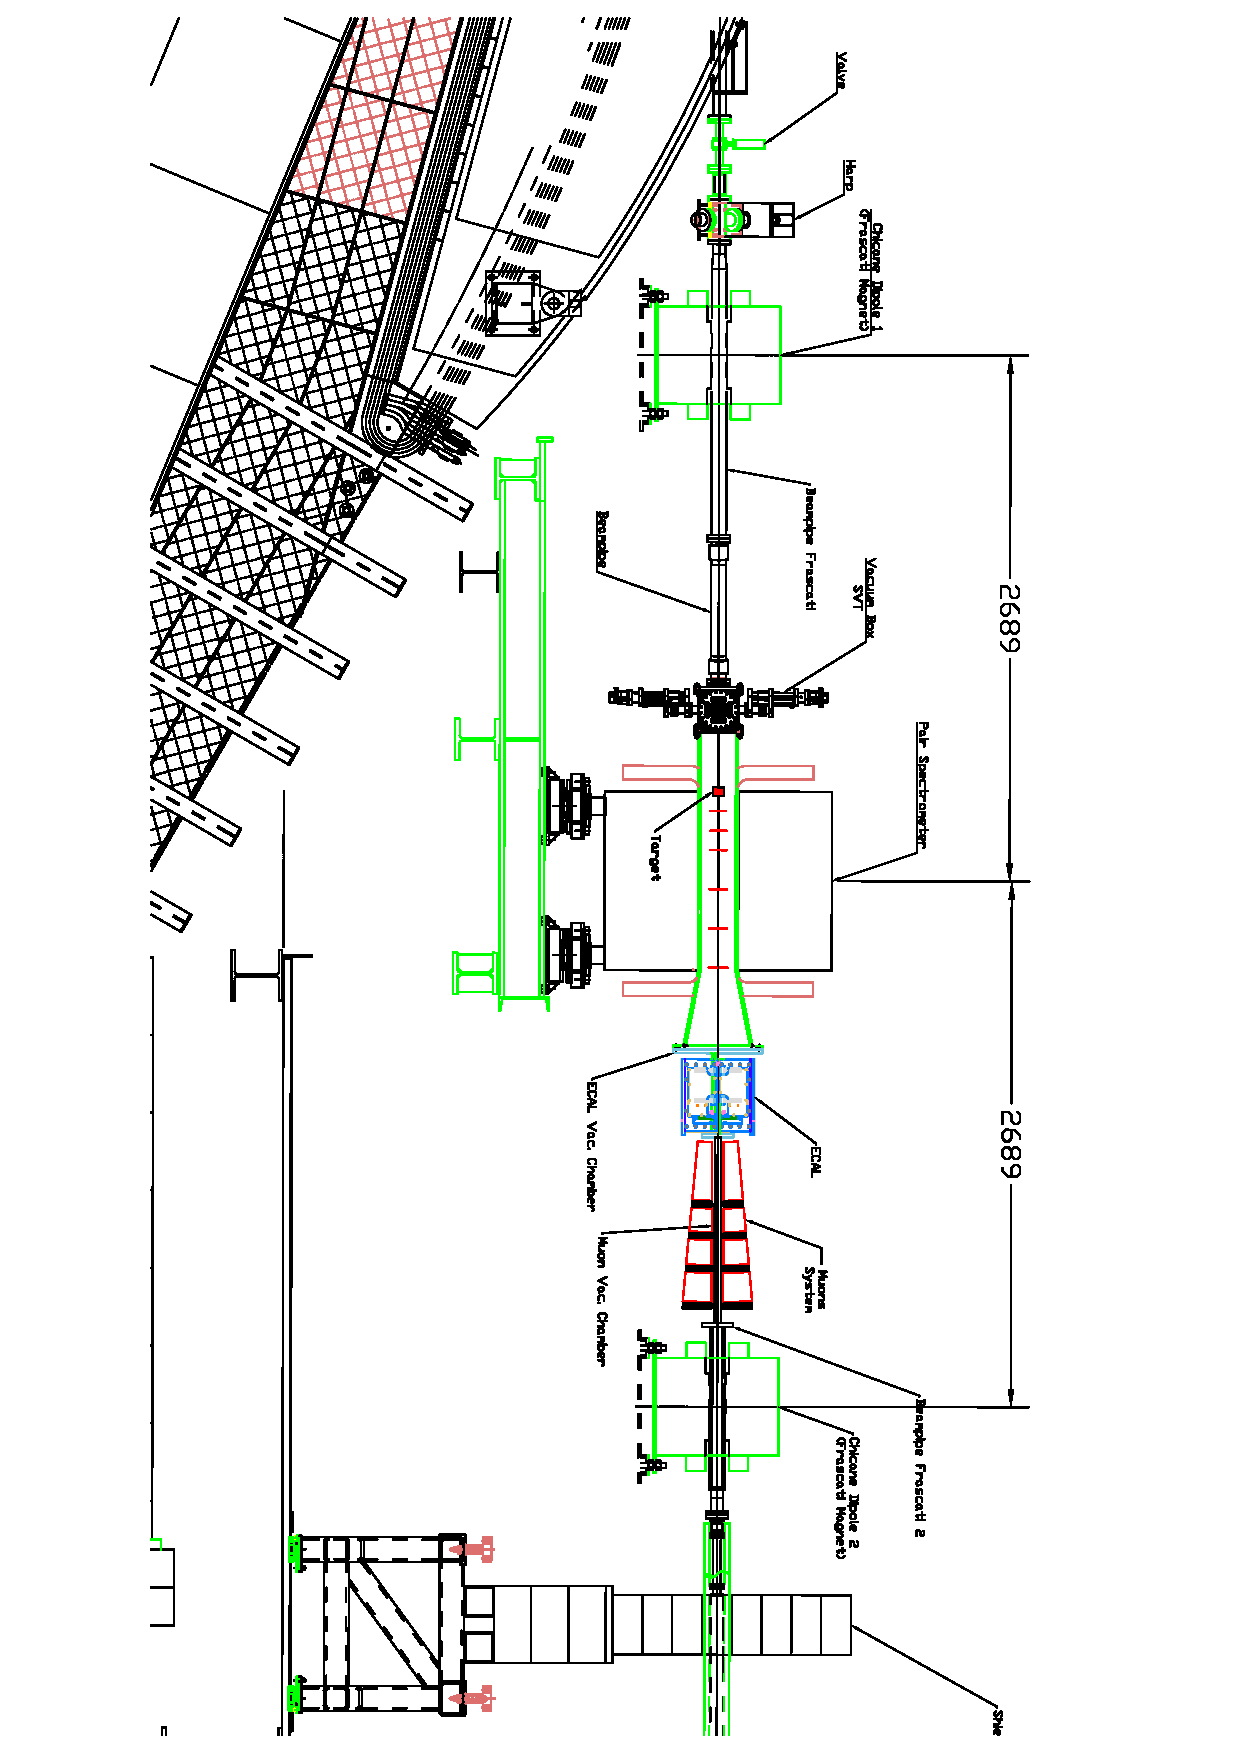
\includegraphics[angle=180, width=0.85\textwidth]{beamline/HPS12_66840e051XX_ELEV.pdf}
\caption{\small{Beam line configuration for the HPS test run with electron beams. Chicane configuration is similar to previously run CLAS experiment.}}\label{fig:ebeam}
\end{figure*}

\begin{figure*}[t]
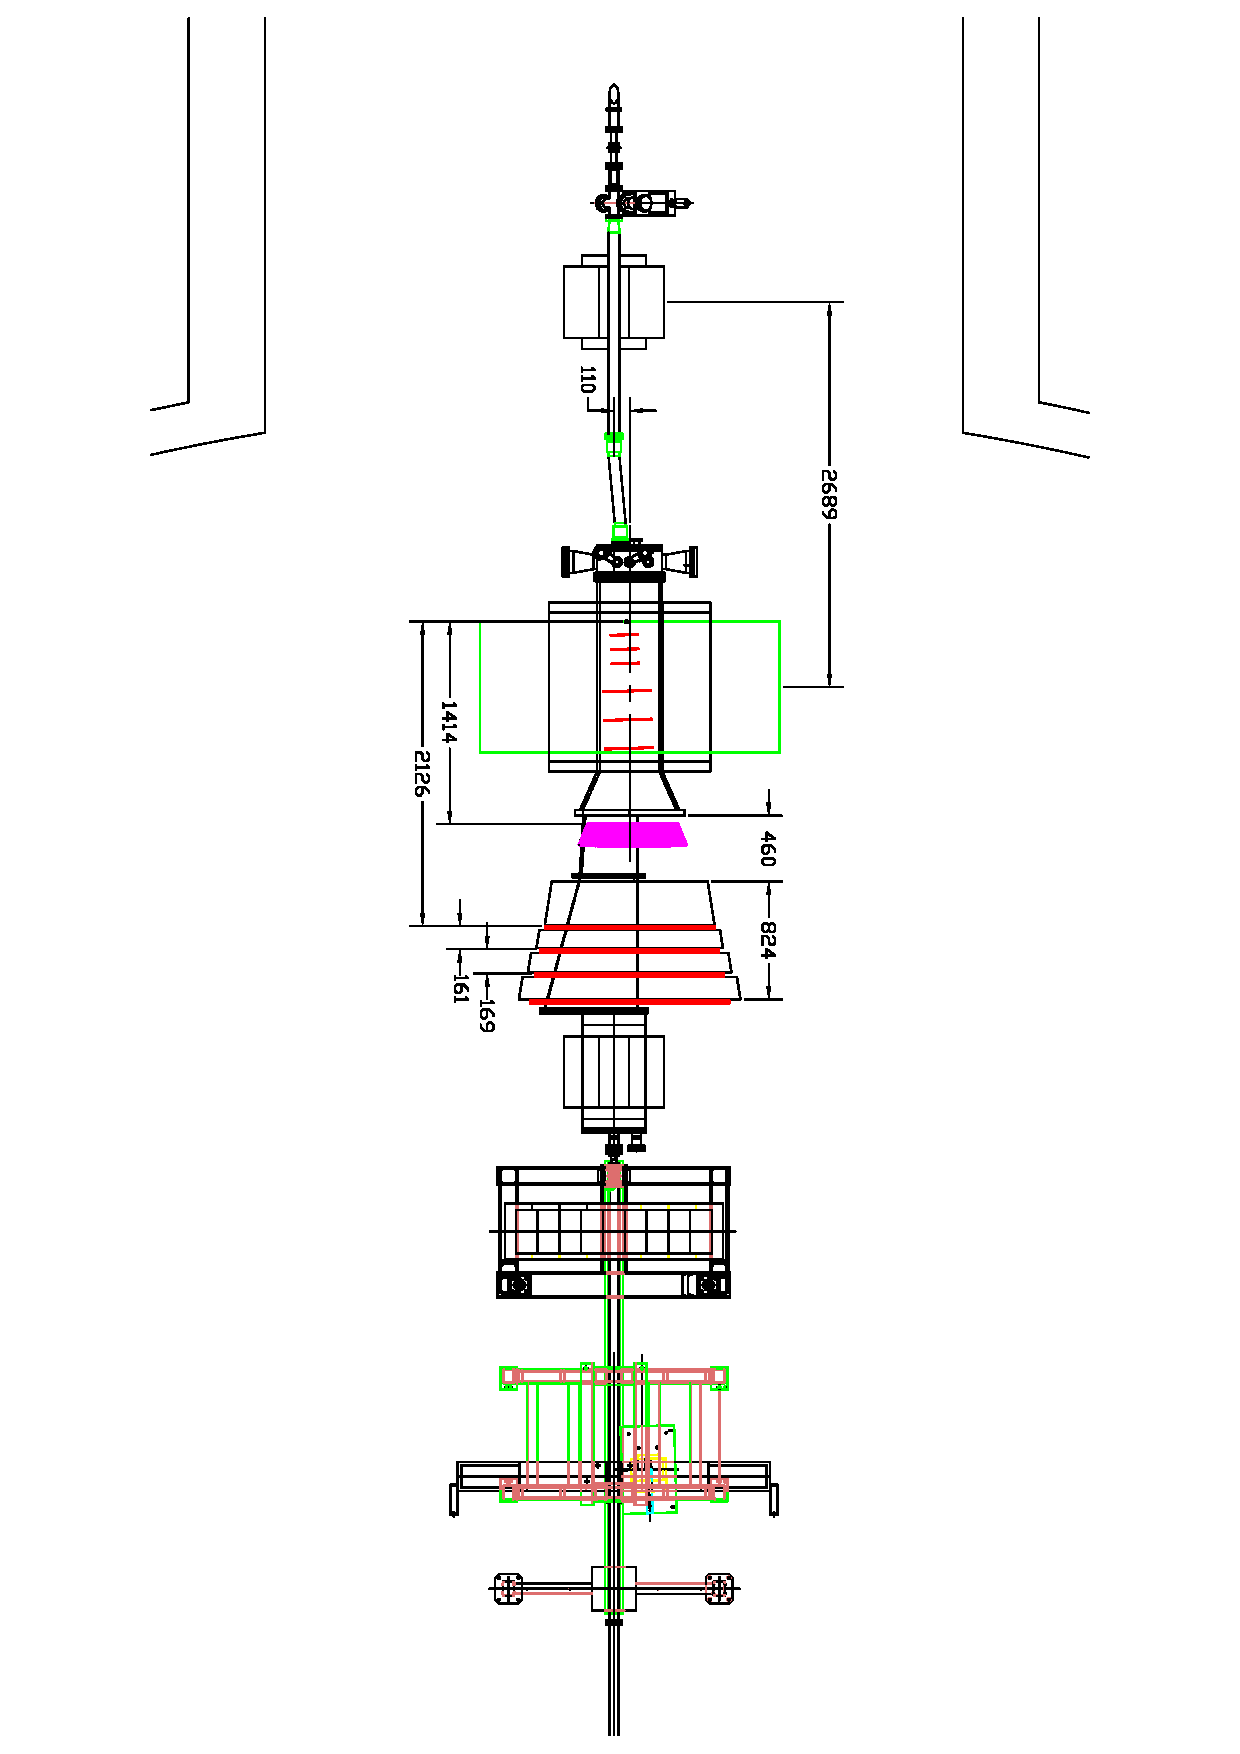
\includegraphics[angle=180., width=0.85\textwidth]{beamline/HPS12_66840e051XX_PLAN.pdf}
\caption{\small{Top view of the beam line configuration for the HPS test run with electron beams. The analyzing magnet is shifted by 4 inches to beam left to get optimal acceptance for both $e^+$s and $e^-$s.}}\label{fig:ebeamt}
\end{figure*}

 
The HPS target is positioned at the upstream edge of the analyzing magnet's pole. The distance from the target to the first layer of the silicon tracker is $10$ cm, and to the face of the electromagnetic calorimeter $\sim 137$ cm. There is continuous vacuum for the electron beam throughout the entire setup ending in the Hall B electron beam dump. The Si-tracker and the target will be located inside the Hall-B pair spectrometer vacuum chamber. The SVT vacuum box is mounted on the upstream end of the analyzing magnet vacuum chamber to provide connections for the SVT motion system, the cooling system, power and signal cables, and the target motion system. The Ecal vacuum chamber is attached to the downstream end of the analyzing magnet vacuum chamber, above and below which are placed the Ecal modules. Downstream of the Ecal vacuum chamber, another vacuum chamber is attached, leading through the muon system and the downstream chicane magnet.

The analyzing magnet, the Hall B pair spectrometer dipole, has its own power supply. The �Frascati� H magnets will use one common power supply and will be powered by the Hall B "mini-torus" power supply. There will be a shunt installed between the two �Frascati� magnets to allow independent small changes in currents on those two magnets if necessary (as it was done during the TPE experiment, although never used). Both power supplies are bipolar, so the magnets can be degaussed when needed. From available field map data at $900$ A, the$\int{Bdl}$ of these magnets along the path of the electron beam is $0.663$ T-m. The specified max current for these magnets is $950$ A. In order to get $0.75$ T-m an additional $10\%$ increase in field value will be needed. From initial evaluation of the magnet design and characteristics, it should not be a problem to run them at $10\%$ higher currents over the specified max current. However, reducing the gap by $1/3$ inch can be done if necessary.

 
\clearpage

\subsubsection{Running Conditions} 
 
The HPS will use $\sim 1.1$ GeV, $\sim 2.2$ GeV, and $\sim 6.6$ GeV electron beams of up to $500$ nA incident on a tungsten (W) target. Operational experience (with 6 GeV) showed that the CEBAF beam is very clean, and is contained within $\pm 0.5$ mm with halo at the level of less than $10^{-5}$. It is expected that behavior of the 12 GeV machine will be understood at the same level, at least for up to 3-pass beams (up $\sim 6.6$ GeV), so there should not be any issue of primary electron beam passing through the �dead zone� gap of the HPS setup. 
 
For checking the vertexing performance and acquiring physics data, an asymmetric beam profile is desirable. Since the vertex resolution in the non-bend plane will be high, beam sizes of $20-30 ~\mu$m in the Y direction are preferable. The momentum measurement will not benefit from small beam sizes in the X direction, and small beam sizes in both dimensions will overheat the target foil. For these reasons the required beam sizes for HPS will be $\sigma_X \sim 250 \mu$m and $\sigma_Y \sim 30 \mu$m.
The HPS beam parameter requirements are presented in Table \ref{tb:beam}. 
 
 \begin{table}[!htb]
 \centering
 \begin{tabular}{|c|c|c|c|c|}
\hline
%Parameter & \multicolumn{3}{c|}{Requirement/Expectation} &Unit \\ \hline 
Parameter & \multicolumn{3}{c|}{Requirement} &Unit \\ \hline 
E & $1100$ & $2200$ & $6600$ & MeV \\ \hline
$\delta$p/p & \multicolumn{3}{c|}{$< 10^{-4}$} & \\ \hline 
Current & $< 200$ & $< 400$ & $< 500$ & nA \\ \hline
Current Instability & \multicolumn{3}{c|}{$< 5$} &\% \\ \hline 
$\sigma_x $& \multicolumn{3}{c|}{$< 300$ } & $\mu$m \\ \hline 
$\sigma_y$&$ < 50$& $ <60$ & $<80$ & $\mu$m \\ \hline
Position Stability & \multicolumn{3}{c|}{$< 30$} &$\mu$m \\ \hline
Divergence& \multicolumn{3}{c|}{$< 100$} & $\mu$rad \\ \hline 
Beam Halo ($> 5\sigma$) & \multicolumn{3}{c|}{$< 10^{-5}$} & \\ \hline
 \end{tabular}
\caption{ Required beam parameters.} 
\label{tb:beam}
\end{table}

The B-line optics in $6$ GeV era was checked using simulation and beam test of the system. The optics program ELEGANT \cite{elegant} was used to determine the optimized B-line parameters needed to achieve an asymmetric beam size, $\sigma_X \approx 250 \mu$m and $\sigma_Y\approx 20 \mu$m, at the HPS test run target location. 
Beam tests were conducted in Hall B to validate these optics simulations during the Two Photon Exchange experiment when $2.2$ GeV beam was available (February of 2011). Parameters were set for a beam profile of $\sigma_X \approx 300 ~\mu$m and $\sigma_Y\approx 10 \mu$m at the Hall B �tagger� beam profiler ($\sim 8$ meters upstream of the proposed HPS target location). Several beam profile scans with different scanner and data readout speeds were performed to check the beam stability and systematics in the measurements. 
One of the scans is shown in Figure \ref{fig:profile_test}. As can be seen from the figure, the required profile can be reliably  achieved. Several scans performed over two hours resulted consistent, stable beam profile. Based on the width of the Y-profile, beam position stability is  $< 20 \mu$m. Note that any beam motion with more than 10 $\mu$m amplitude and faster than 1Hz is included in the scan.

\begin{figure*}[t]
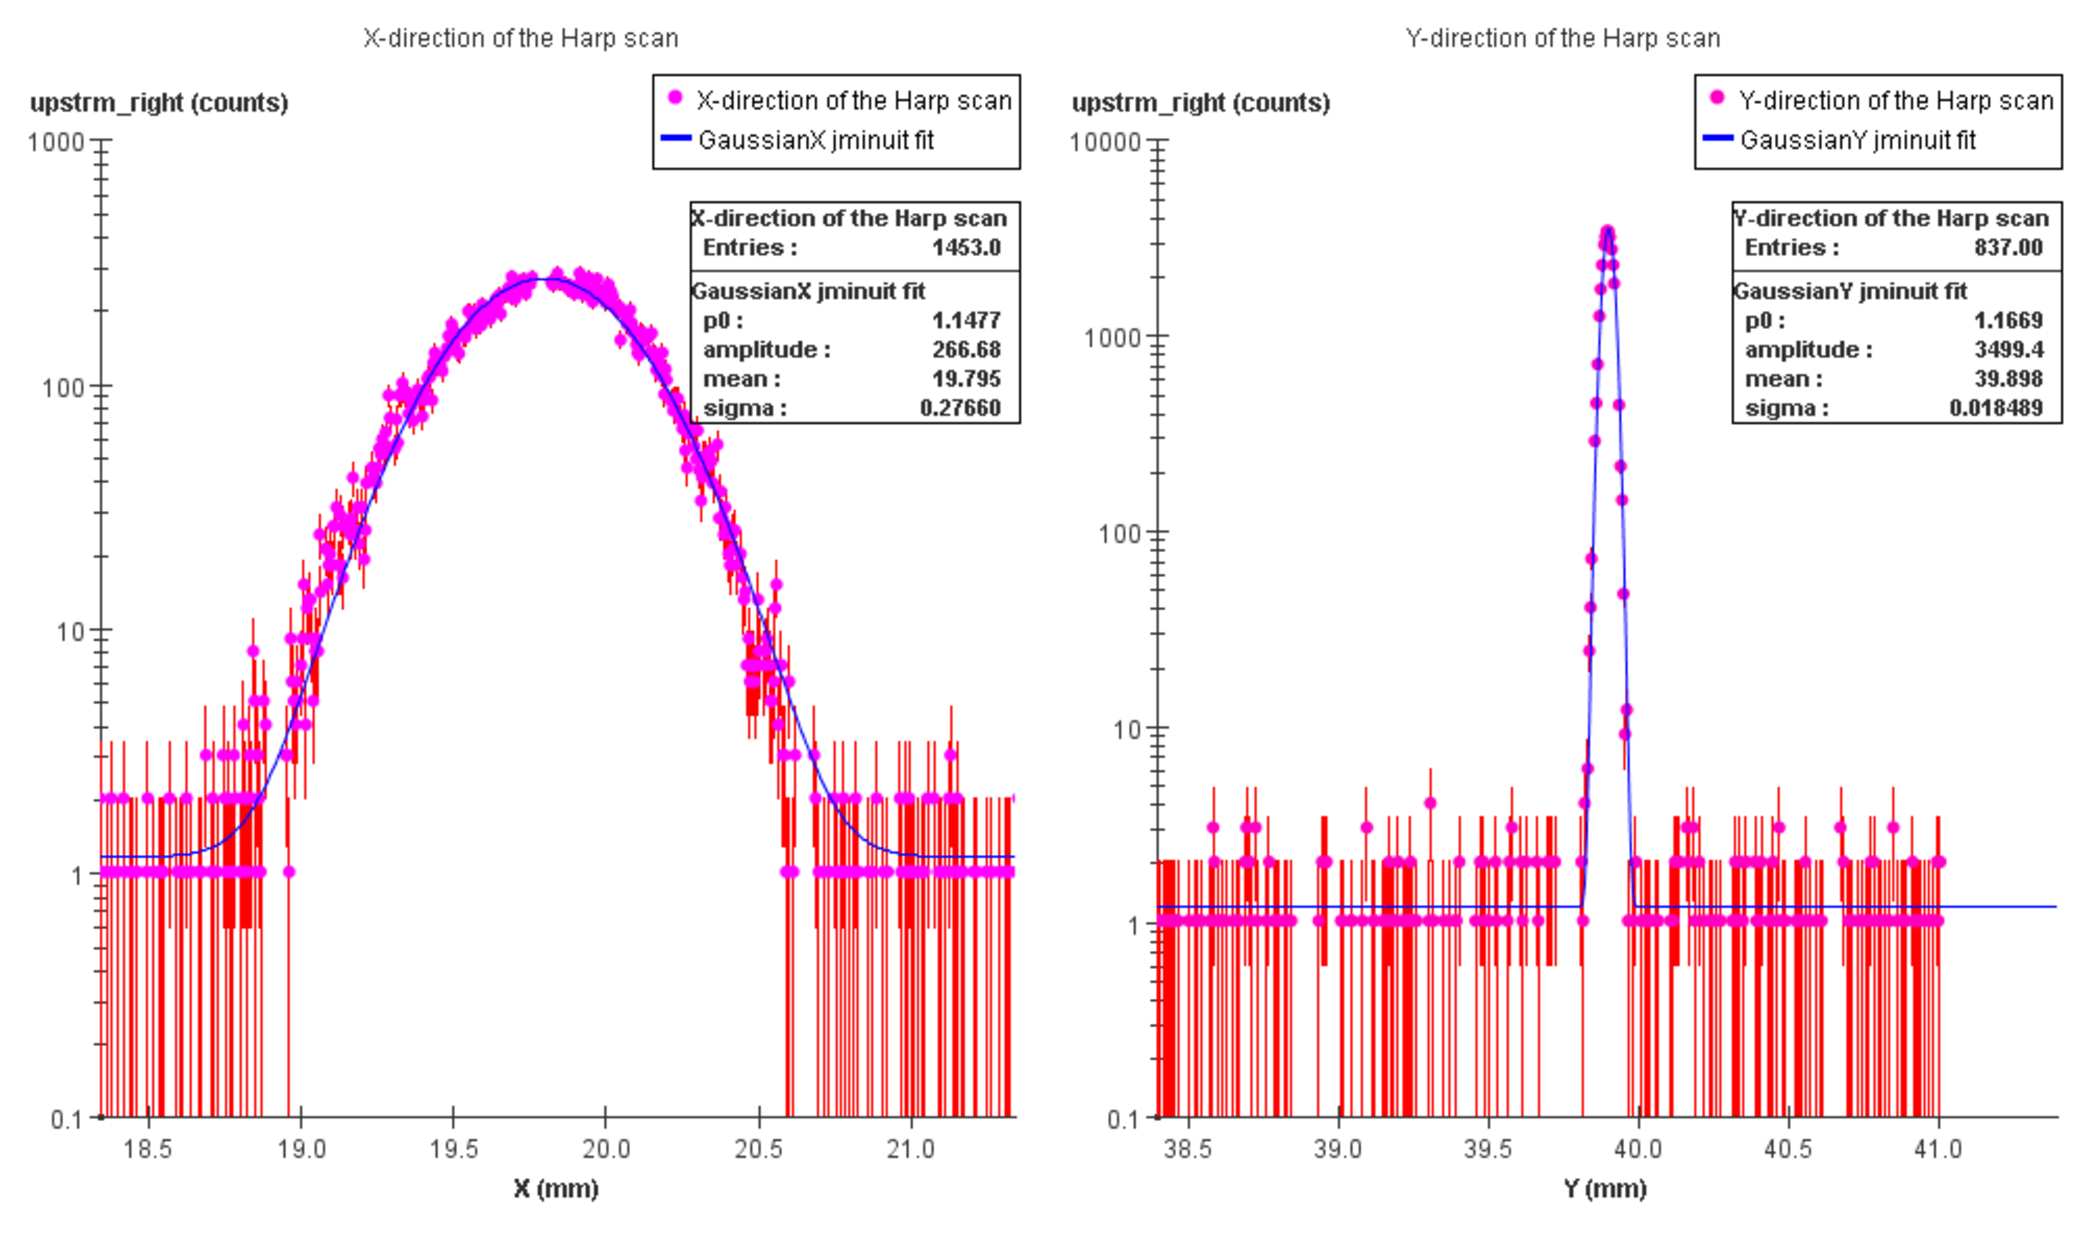
\includegraphics[scale=0.45]{beamline/harp_02.pdf}
\caption{\small{Wire harp scan after loading optics parameters from optimization using ELEGANT program. The wire scan speed was 0.1mm/s, readout speed is 15Hz. Based on the width of the Y-profile, beam position stability is  $< 20 \mu$m. Note: any beam motion with more than 10 $\mu$m amplitude and faster than 1Hz is included in the scan.}}\label{fig:profile_test}
\end{figure*}
 
% {\bf {\it ELEGANT for 12 GeV machine} from Arne}
The beamline optimizations have been performed for 12 GeV CEBAF machine with proposed changes for Hall-B/CLAS12 operations. Using program ELEGANT and the new location of magnetic elements and their field maps beam profile was optimized at the HPS target location. In Figure \ref{fig:hps2014} the beam sizes and the beam angles are shown for $6.7$ GeV setup.  Required beam size is achievable within specifications of all quadropoles.  Since HPS will run at beam energies $<6.7$ GeV it is straight forward to scale (linearly) the magnets down to the other energies.  The beam size/angle (beam transport) remains the same for $1.1$, $2.2$, and $4.4$ GeV energies with the exception of the small emittance increase at $6.7$ GeV.
  
  \begin{figure*}[t]
%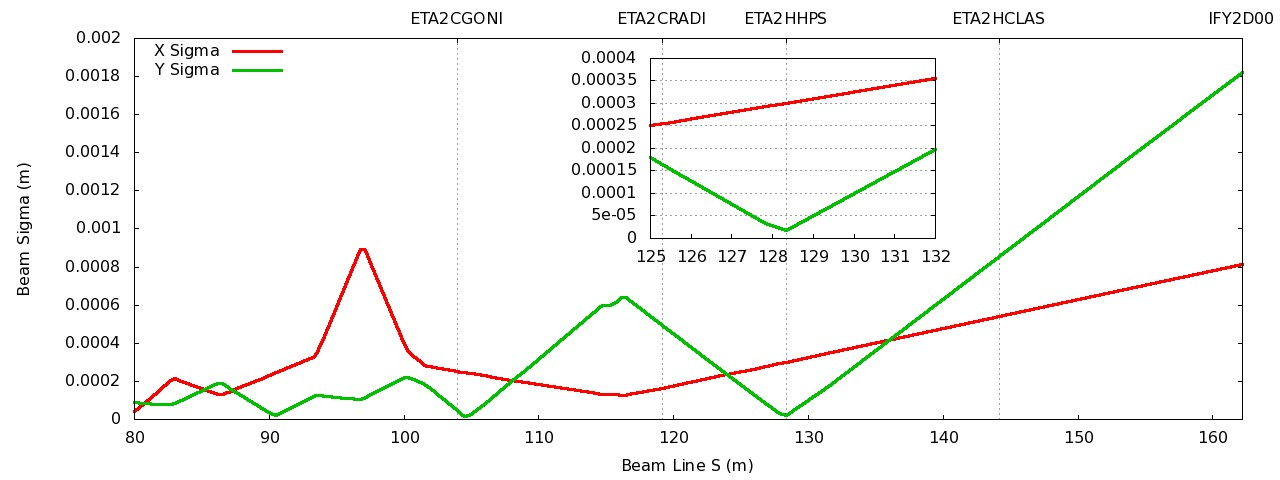
\includegraphics[scale=0.35]{beamline/hps_test_300_by_15.jpg}
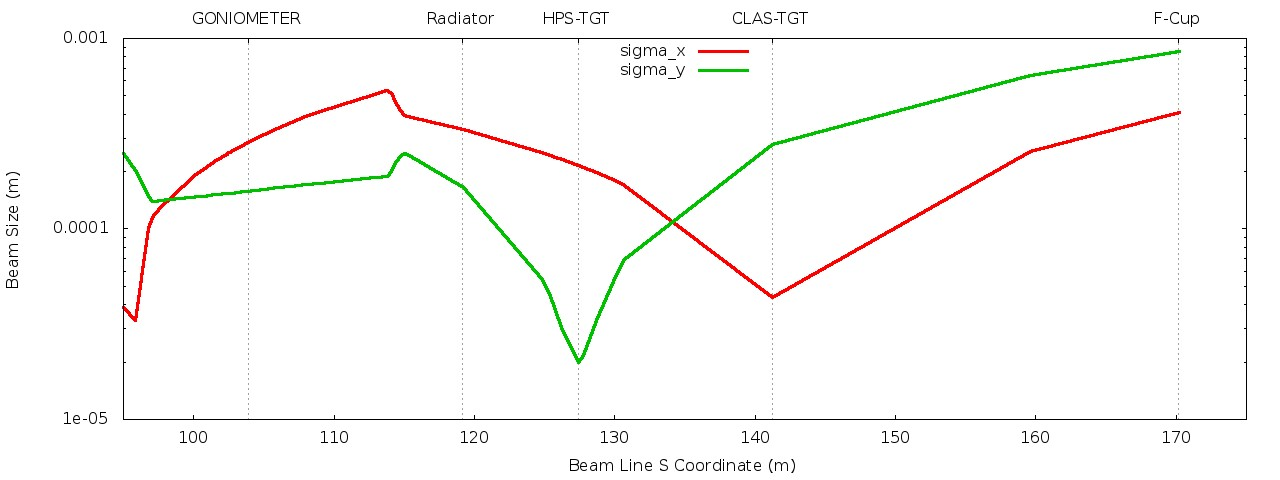
\includegraphics[scale=0.35]{beamline/hps2014_beamsize.jpg}
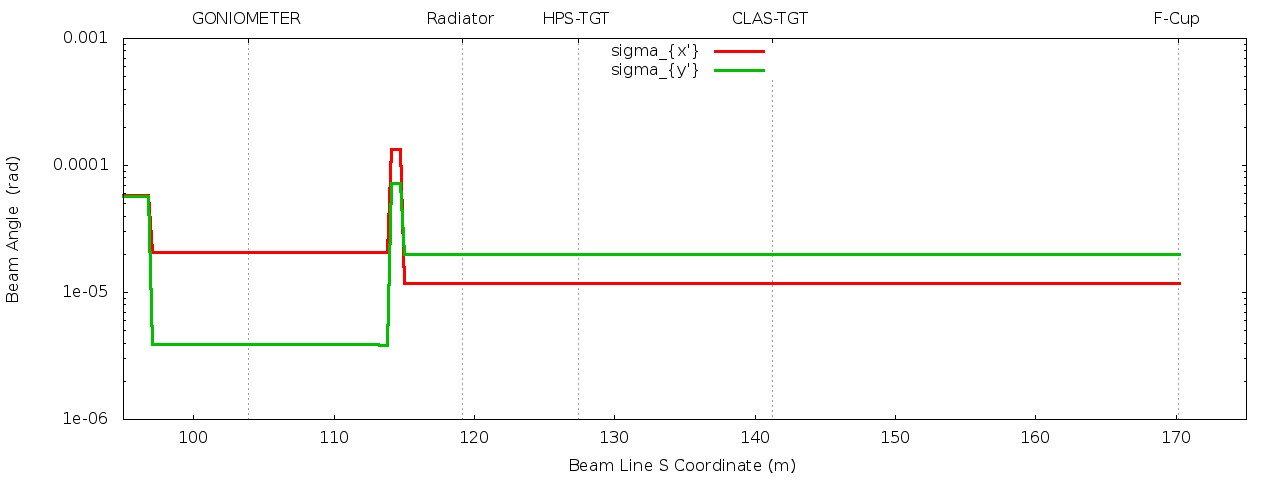
\includegraphics[scale=0.35]{beamline/hps2014_beamangle.jpg}
\caption{\small{Beam sizes in X and Y along the B-line in the upstream tunnel and in the region of the HPS test run setup. At the HPS target asymmetric beam profile $\sigma_X=300 \mu$m and $\sigma_Y=20 \mu$m can be achieved with existing B-line optics.}}\label{fig:hps2014}
\end{figure*}


 
 \subsubsection{Beam Diagnostics}
 
Beam position and current will be controlled by two sets of cavity beam position monitors (BPMs), that are located in the upstream tunnel. Sets of corrector dipoles and quadrupoles are routinely used to tune the beam for Hall B (2C21 to 2C24). A pair of BPMs, 2C21 and 2C24, will define the incoming trajectory of the beam and are included in the fast feedback loop. Readings from these BPMs will be used to maintain stable beam positions and currents. The stability of beam positions at two different locations also ensures the stability of the beam inclination.
 
The beam profile will be measured using three wire scanners, two installed in the tunnel, first one at 2C23, the second one before the Hall-B tagger magnet, (2c24 harp, called "tagger harp"), about 8 meters upstream of the HPS target. The last wire harp, 2H00 harp, will be located just before the first chicane dipole . First two profilers will be used to establish the required beam parameters during the initial setup. The Hall-B tagger magnet will be energized when beam tune is in progress. After acceptable beam profile is achieved, beam will be put through the HPS system (tagger magnet will be degaussed and turned off) and beam profile will be checked using 2H00 wire harp. The backgrounds in the HPS silicon tracker from beam profiling using the 2H00 harp has been simulated. At $5$ nA beam current, the radiation damage is equivalent to about $10$ sec. of production beam current on the target.

An insertable YAG screen beam viewer will be installed in the downstream alcove of Hall-B, before the Faraday cup, $\sim 40$ meters downstream of the HPS target. Both position and profile of the beam will be used to setup the chicane magnets and to monitor beam quality during the run. A set of beam halo counters mounted along the beam line provides continuous and fast monitoring of the beam conditions. These counters are like those used for beam profile measurements. Excess noise in the beam halo counters triggers the machine fast
shutdown system (FSD) in order to terminate beam in the event of beam excursions which could damage the HPS detectors. The FSD will occur in less than 50 $\mu$s. In addition to halo counters, a beam offset monitor (BOM) will be installed upstream of the 2H00 wire harp. It is similar to BOM used in CLAS. A short quartz cylinder, about $1$ cm in diameter, with optical fibers attached around the edge will be centered on the beam. Few electrons on the beam tail will generate light in the cylinder that will be detected in a multi-anode PMT attached to readout fibers. Any beam motion towards the collimator located upstream of the tagger magnet will generate more light and increase the counts in the PMT scalers. BOM will be wired to FSD as part of the equipment protection system. 
 
\subsubsection{Vacuum chambers} 
\label{vacchamb}
 
The SVT vacuum box will be attached to the existing magnet vacuum chamber as shown in Figure \ref{fig:svtvbox}. Power, high voltage, and data signals to and from the hybrids are connected through two $8$" flanges on the sides of the vacuum box. Two vertical linear motion mechanisms driven by stepper motors 
are used to position the SVT upper and lower modules with a precision of $1.25 ~\mu$m/step. A third linear motion mechanism is used to position the target on or off the beam. All the stepper motors are placed at a large enough distance from the magnet to avoid any ill effect from the magnetic field.
An existing stepper motor driver and  EPICS-based control software will be used.   
 
\begin{figure*}[t]
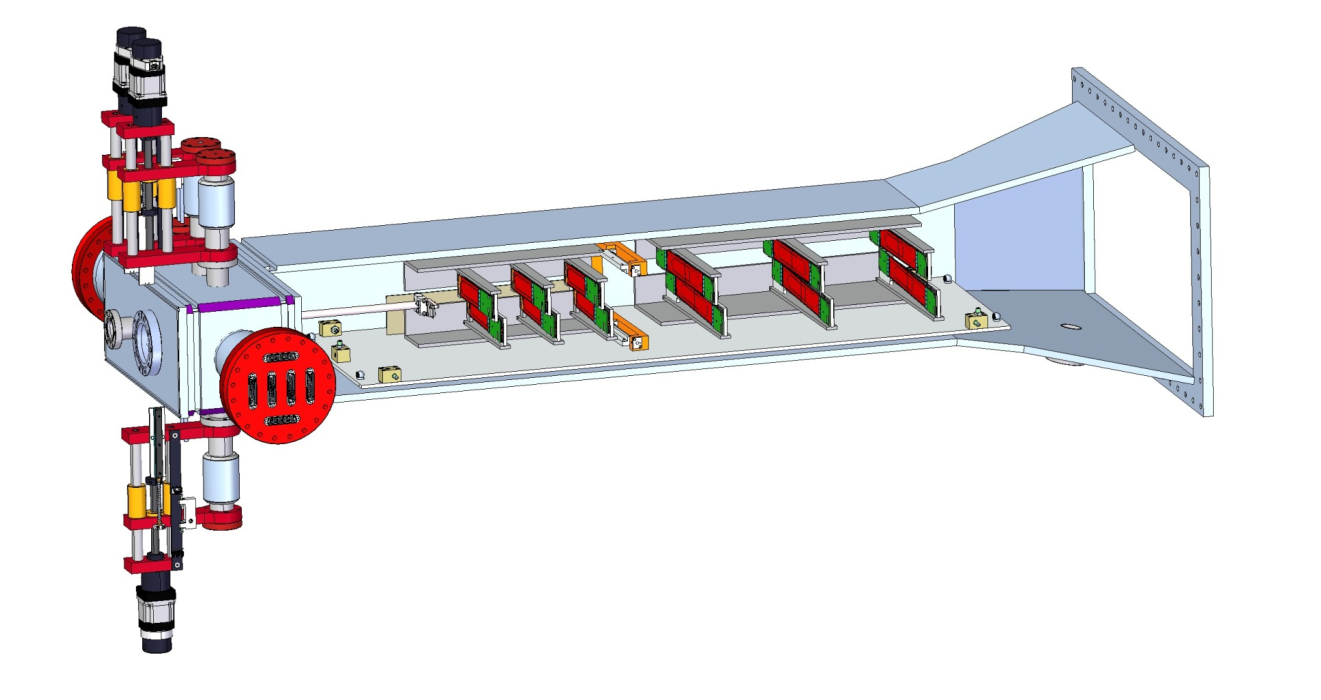
\includegraphics[scale=0.75]{beamline/svt_in.pdf}
\caption{\small{Rendering of the SVT inside the Hall-B pair spectrometer vacuum chamber and the upstream vacuum box with SVT and target connections.}}\label{fig:svtvbox}
\end{figure*}

The scattering chamber between the top and bottom parts of the ECal is a critical beamline element. In order to keep the calorimeter as close as possible to the beam plane, include sufficient thermal insulation for the ECal, and maintain as wide a vacuum gap as possible, the top and bottom plates of the scattering chamber must be quite thin. At the location where the primary beams  ($e^-$ and $\gamma$) exit, the openings in the chamber have been enlarged. In Figure \ref{fig:ecalv} a rendering of the scattering chamber in between two halves of the ECAL is shown. The front flange of the chamber connects directly to the magnet vacuum chamber. Vacuum is maintained only on the electron side (beam right).  This design is based on detailed GEANT4 simulations of background rates and acceptance of the ECal and allows crystals to be within 20 mm from the beam plane. In order to avoid excessive deformation of the thin walls of the vacuum chamber, an aluminum honeycomb support is inserted between the upper and lower walls, to beam's right.

The ECal vacuum chamber will be continued with a scattering chamber between two halves of the muon system. The openings for the photon and electron beams will not be necessary. The gap for the radiated secondary electrons will be projections of the ECal vacuum chamber. At upstream end muon vacuum chamber will have uniform gap of $\sim 4$ cm. At the downstream end that gap will be $\sim 5$ cm.

The last scattering chamber, through the third dipole, does not need to have narrow opening, it will have size of the Frascati H magnet gap. At the end of the vacuum chamber there will be flange with two exit windows, a Kapton window for photon beam to exit the chamber and go to the photon beam dump through a Helium bag, and a vacuum continuation to the standard beam line for the electron beam to go to the Hall-B electron beam dump. 

\begin{figure*}[t]
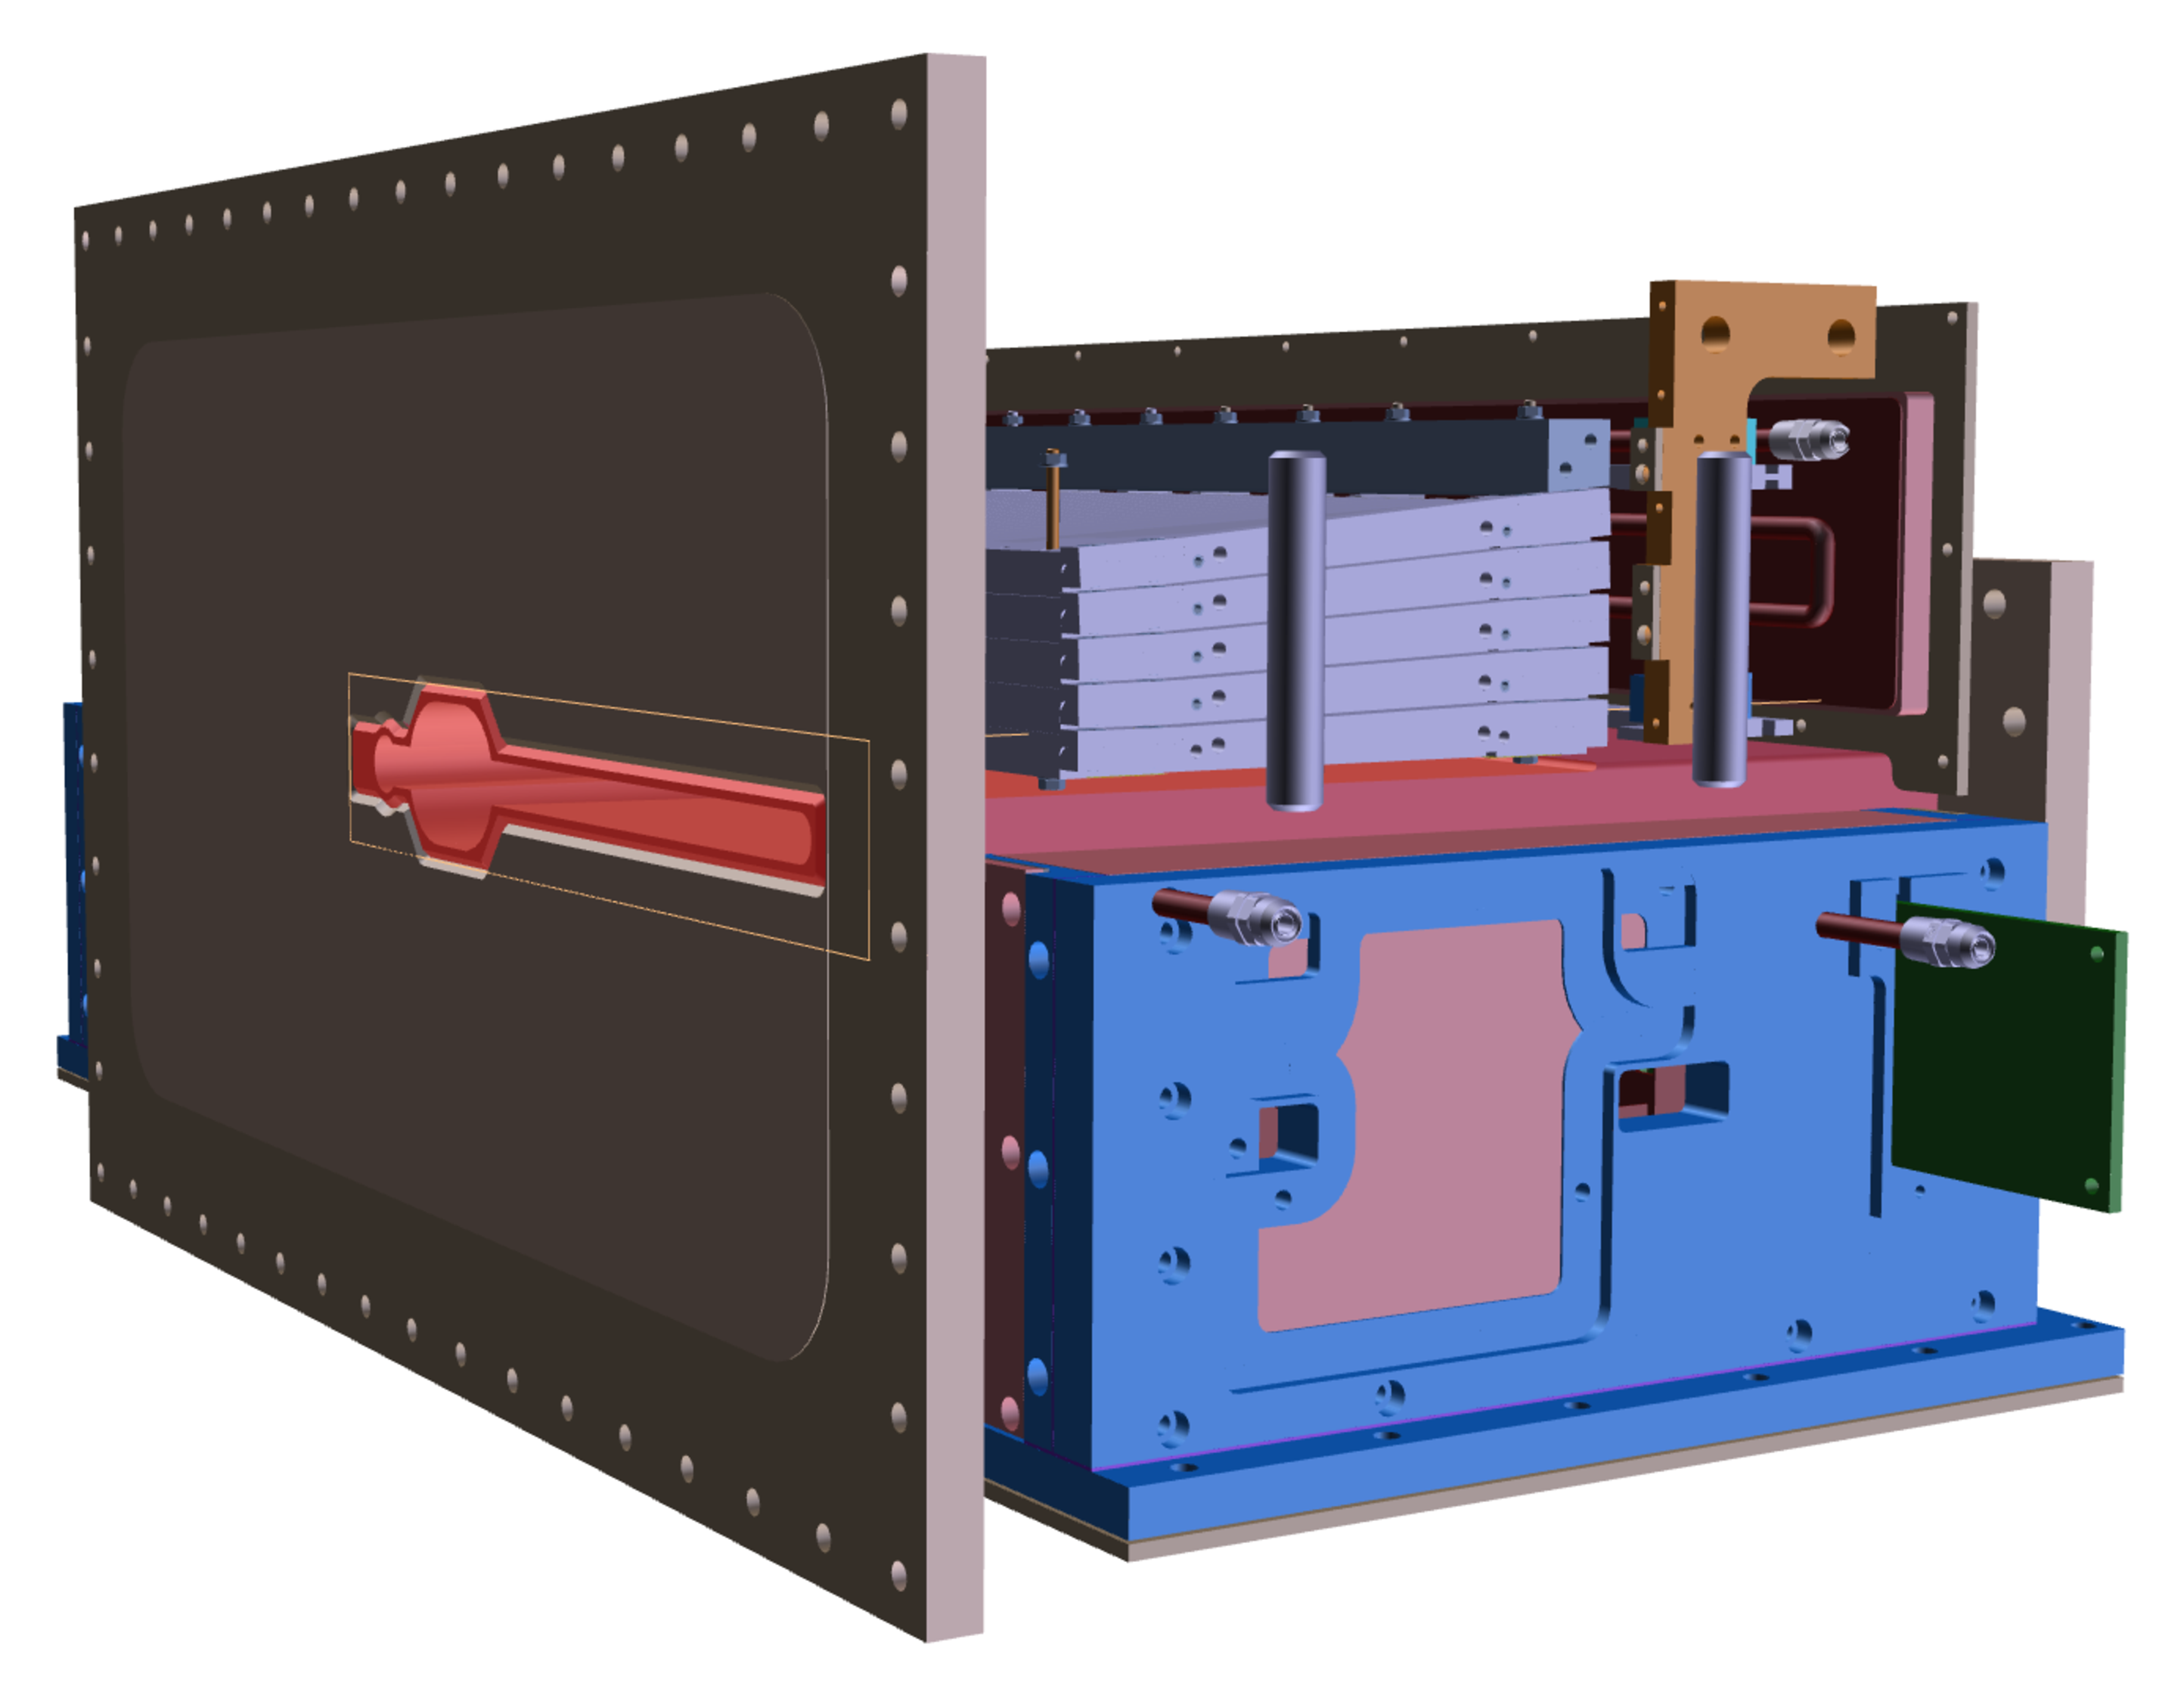
\includegraphics[scale=0.25]{beamline/ecal_vac.pdf}
\caption{\small{Rendering of the ECal and the ECal vacuum chamber.}}\label{fig:ecalv}
\end{figure*}
 
\subsubsection{Beam dumps and shieldings} 

The Hall-B electron beam dump will be used to terminate the electron beam. Due to the high intensity beam will not be dumped on Faraday cap (FC), instead, the existing beam blocker before the FC will be used to terminate the beam. The photon beam will be dumped in a photon beam dump, which will be a hat  made of lead bricks located on the space frame. There will be a shielding wall after the last chicane magnet to prevent radiation from reaching to detector systems downstream side of the Hall.

\subsubsection{Targets} 
\label{target}

A thin tungsten foil is used as the target. High Z material is
chosen for its short radiation length, to minimize the hadronic
production relative to the electromagnetic trident and A'
production. The target is located 10 cm in front of the first
plane of silicon strip detectors.

The primary target, 10 mm square, is 0.00125 radiation lengths
(approximately 4 $\mu$m tungsten). Mounted immediately above it
is a similar area of 0.0025 radiation lengths, available for some
of the data taking, adjusting the beam current as appropriate.
The foil can be fully retracted from the beam, and is inserted on
to the beam line from above, using a stepping motor linear
actuator. The bottom edge of the foil is free-standing so there
is no thick support frame to trip the beam when the target is
inserted. Its position is adjustable vertically allowing either
thickness to be selected, and different sections of the
tungsten can be used in the event of beam damage. The support
frame on the beam-right side of the target is made thin enough to
prevent radiation damage to the silicon in the event of an errant
beam caused, for example, by an upstream chicane magnet trip.
               
The target is intended to operate with beam currents up to 450
nA, which produce strong local heating. The strength of tungsten
drops by an order of magnitude with temperature increases in the
range of 1000 C. In addition, the material re-crystallizes above
this range, which increases the tendency for cracking where
thermal expansion has caused temporary dimpling. For these
reasons, it was decided to keep the temperature rise less than
about 1000 degrees, which is accomplished by selecting an
adequately large beam spot area. For example at 200 nA the rms
beam radii will be held above 20 by 250 $\mu$m, or 40 by 250
$\mu$m for 400 nA. Simulations have shown that these beam spot
sizes do not diminish the pair reconstruction resolution of the
experiment.

In addition to the target, a set of tungsten beam-fiducial wires
will be installed immediately in front of the silicon detectors.
One horizontal wire, 20 $\mu$m diameter, and one 30 $\mu$m wire
at 9 degrees to the horizontal, will be mounted on a frame
attached to the upper movable silicon support plate, and
similarly for the bottom plate. The frames for the wires are wide
enough that they do not occlude the silicon active area. The
wires can be used to locate the position of the beam relative to
the silicon. To accomplish this safely, the vertical separation
between the front silicon sensor and its nearest wire is 8 mm.
This separation, and their small diameters, also means that, when
the sensors are positioned for data taking, the wires have a
negligible effect on acceptance. The wires are also available for
use as a fairly conventional wire scanner. In particular
they can provide information about the minor and major axes, and
the tip angle (roll), of a strongly elliptical beam.

 
